\documentclass{article}
\usepackage[utf8]{inputenc}
\usepackage{graphicx}
\graphicspath{ {img/} }
\begin{document}

\title{GroundsBot:Autonomous Golf Course Maintenance}
\date{September 2017}
\author{Team A        \\ David Evans \\
        Adam Driscoll \\ Henry Chen  \\
        Josh Bennett  \\ Joe Phaneuf \\ }
\maketitle
\newpage

\tableofcontents
\newpage

\section{Project Description}
GroundsBot \\
\subsection{Functional Requirements}
Groundsbot shall:
  Receive mowing regions
  Cut grass at the correct height
  Create a mowing plan
  Cut the rough 
  Avoid obstacles
  Provide feedback to the groundskeeper
\begin{center}
\begin{tabular}{ |c|c|c| }
  \hline
    M.P1 & Req 1 & My First Requirement \\
    D.P1 & Req 2 & My Second Requirement \\
  \hline
\end{tabular}
\end{center}

\subsection{Non-Functional Requirements}
M.N.1 Bot has emergency stop
M.N.2 Bot is clearly visible/noticeable
M.N.3 Bot does not destroy grass
D.N.1 Operates in variable lighting conditions
D.N.2 Deck adjustable 0.5” to 2”
D.N.3 Survives deluge of golf balls


\subsection{Performance Requirements}
M.P.1 First time user inputs map within 15 minutes
M.P.2 System returns proposed route/coverage map within 5 minutes
M.P.3 Cut 0-25% overlap for 95% of grass
M.P.4 Mow 50 ft^2 of 30 degree sloped grass
M.P.5 Detect 80% of objects greater than 27 cubic inches
M.P.6 Mow to within 1 foot of detected obstacles
M.P.7 Mow 90% of a ¼ acre area

D.P.1 Mow to within 3 inches of a detected obstacles
D.P.2 Return home to within 5 feet of start
D.P.2+ Return home to and mates with a charging dock
D.P.3 Visually report mowing mowing coverage and known obstacles

\section{Use Case}

\section{System Level Requirements}
Objective Tree
Work with existing operations
  Minimal installation effort
  Operate with minimal intervention
  Allow for machine maintenance

Upholds golf course standards
  Operates safely 
  Reflects golfing aesthetics
  Low impact on golfers
  
Reduce net rough maintenance cost
  Reduce manual labor
  Reduce ammmortized cost per acre
  
\subsection{Chassis and Drivetrain}
\subsection{Sensor Suite}

\section{Functional Architecture}
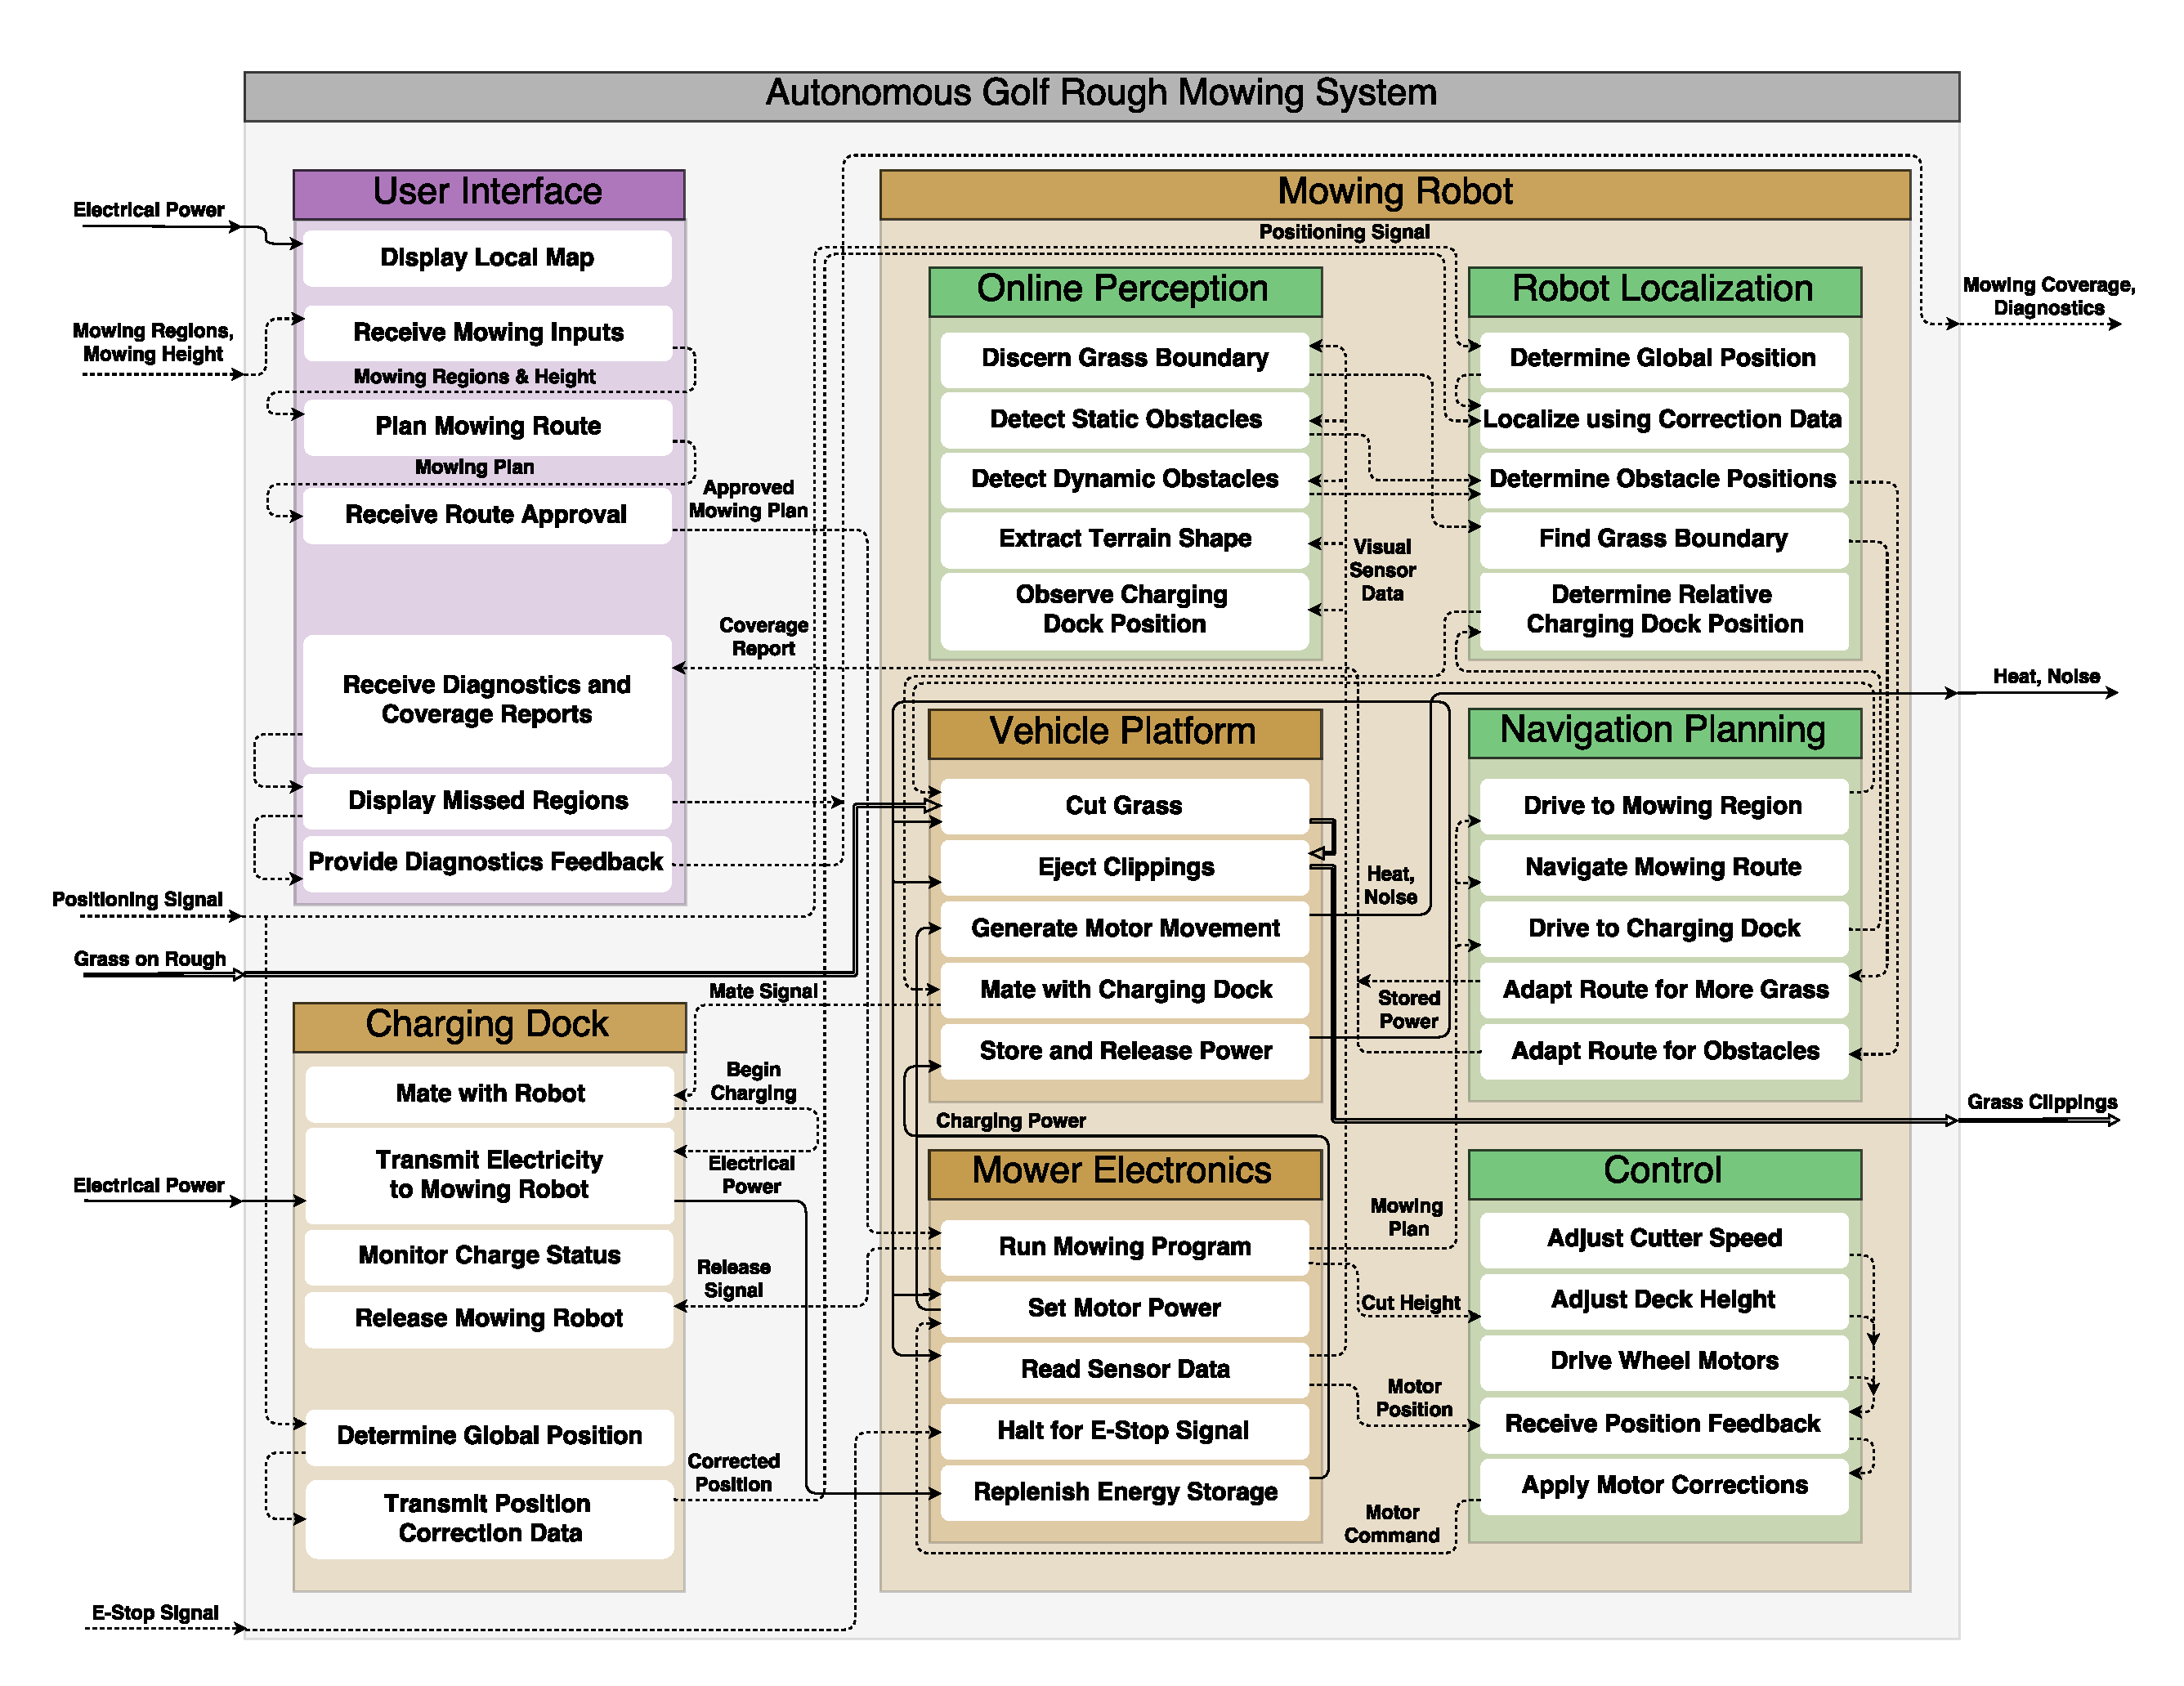
\includegraphics[scale=0.3]{functional}

\section{System Level Trade Studies}

\section{Cyberphysical Architecture}
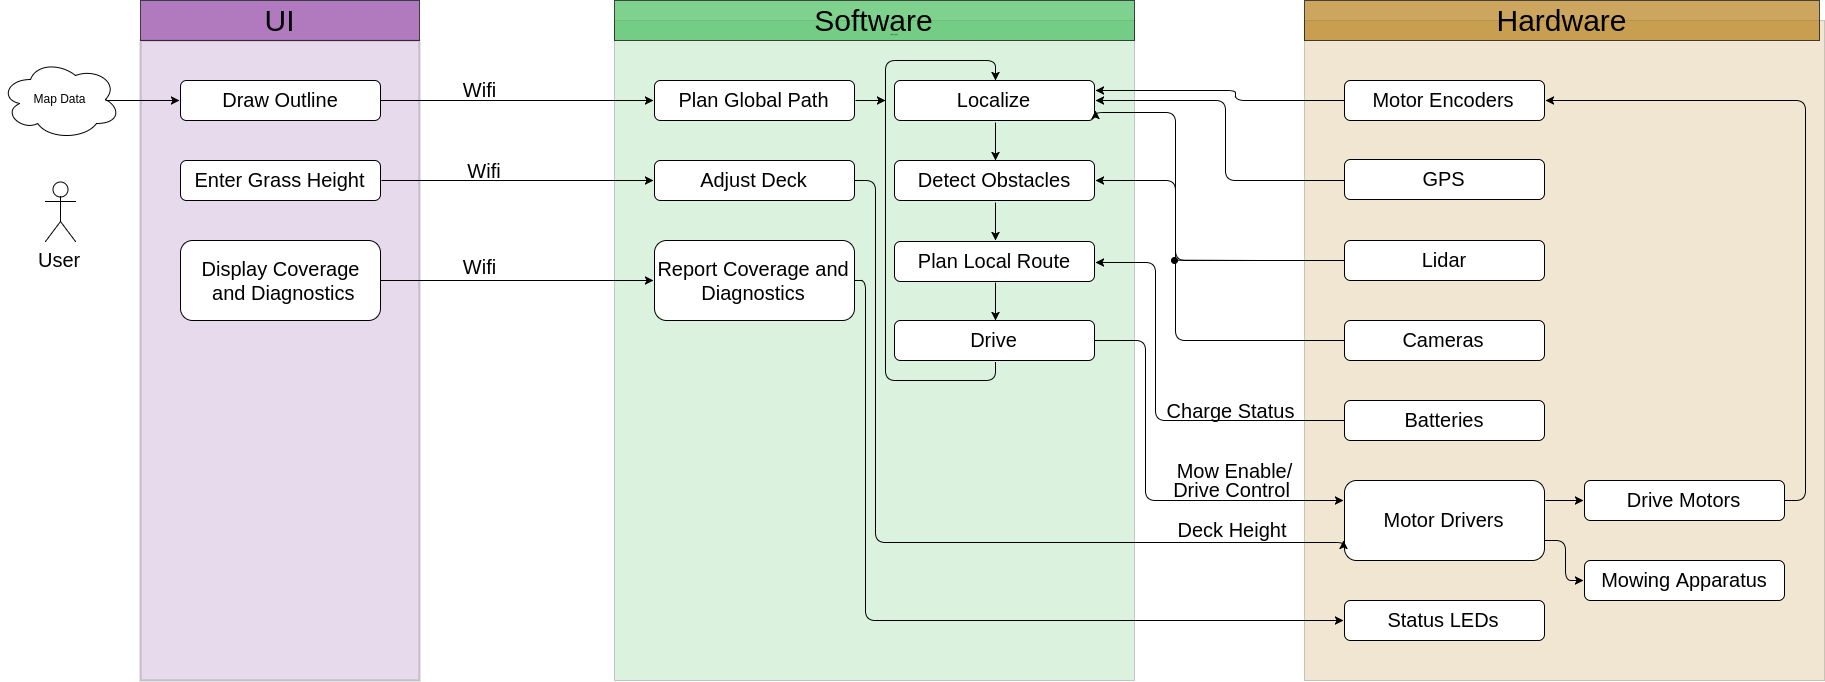
\includegraphics[scale=0.2]{cyberphysical}

\section{Subsystem Descriptions}

\section{Project Management}

\section{References}

\end{document}
